\documentclass{article}
\usepackage[margin=1in]{geometry}
\usepackage{tabulary}
\usepackage{float}
\usepackage{lipsum}
\usepackage[utf8]{inputenc}
\usepackage{hyperref}
\usepackage{graphicx}
\usepackage{graphics}
\usepackage{listings}
\lstset
{ %Formatting for code in appendix
    language=C,
    basicstyle=\small,
    numbers=left,
    stepnumber=1,
    showstringspaces=false,
    tabsize=1,
    breaklines=true,
    breakatwhitespace=false,
}
\usepackage{xcolor}
\lstset{escapeinside={<@}{@>}}
\usepackage[T1]{fontenc}
\usepackage[parfill]{parskip}
\newcommand{\code}[1]{\textsf{#1}}
\setlength{\parindent}{0em}
\begin{document}
\begin{center}{\LARGE CS406: Compilers} \end{center}
\begin{center}{\large Programming Assignment 4: Statements and Expressions,  Due: 20/3/2020} \end{center}

\bigskip



\section{Introduction}
Your goal in this step is to generate executable code for statements (assignment, READ/WRITE) and expressions.
To do this, you will build semantic actions that generate code in an {\em intermediate representation} (IR) for assignment statements and expressions, and then translate that intermediate representation to assembly code.
We recommend that you do this in three steps, as it will make it easier to debug your code, but you can also choose to do it in two steps (step 1 is optional):
\begin{enumerate}
	\item Generate an {\em abstract syntax tree} (AST) for the code in your function.
	\item Convert the AST into a sequence of IR Nodes that implement your function using three address code.
	\item Traverse your sequence of IR Nodes to generate assembly code.
\end{enumerate}

(Note: in this step, and step 5, we will only have one function in our program, main.)

\section{Abstract Syntax Tree}
An Abstract Syntax Tree is essentially, a cleaned up form of your parse tree that more straightforwardly captures the structure of expressions, control constructs, etc. in your program. For many compilers, the AST {\em is} the intermediate representation, though we will further convert the AST into another intermediate representation.

\paragraph{What is the difference between a parse tree and an AST ?}
Parse trees capture all of the little details necessary to implement your grammar. This means that it often contains extraneous information beyond what is necessary to capture the details of a piece of code (e.g., there are nodes for tokens like ``;'', and nodes for all of the sub-constructs we used to correctly implement order of operations). ASTs, in contrast, contain exactly the information needed to capture the meaning of an expression, including being structured to preserve order of operations.

For example, consider the parse tree for \texttt{a + b * c}:

\begin{figure}[H]
	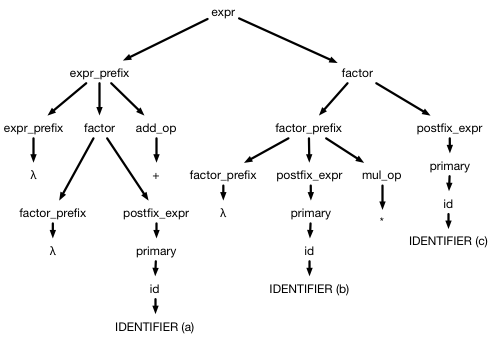
\includegraphics[scale=0.5]{parsetree}
\end{figure}

Complicated, huh? Here's an abstract syntax tree that captures the same thing:

\begin{figure}[H]
	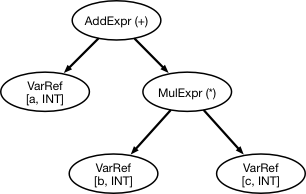
\includegraphics[scale=0.5]{ast}
\end{figure}

Much simpler! We aren't preserving anything except the bare minimum needed to describe the expression (note that we included the type of each of the variables in the program -- we can get that information from our symbol table!).
Building an AST

\subsection{Building an AST}
Note that the information in the AST is associated with various nodes in the parse tree. We can use semantic actions, just as we did in Step 3, to pass information ``up'' the parse tree to build up the AST. Instead of passing information about a declaration, we can instead pass partially constructed abstract syntax tree nodes (you may want to define a class or structure called \texttt{ASTNode} that can be the ``return type'' for the relevant constructs). For example:

\begin{itemize}
	\item \texttt{add\_op} : generate an \texttt{AddExpr} AST node that has two children (that you leave uninitialized) and keeps track of the operator (+ or -).
	\item \texttt{expr\_prefix}: this will have three AST Nodes passed up from its sub rules: one from \texttt{expr\_prefix} (which may be NULL, but otherwise will be an \texttt{AddExpr} node missing its right child), one passed up from \texttt{factor} (which will be a complete AST Node with all its fields filled in), and one passed up from \texttt{add\_op} (which will be an \texttt{AddExpr} node that has neither its left nor its right child filled in). 
		\begin{enumerate}
			\item If \texttt{expr\_prefix} is NULL, make the \texttt{add\_op} node's left child the node from \texttt{factor} and return up the \texttt{add\_op} node (note that it won't have its right child filled in!)
			\item If \texttt{expr\_prefix} isn't NULL, note that it will be missing its right child. Make the \texttt{factor} node its right child, then make the \texttt{expr\_prefix} node the \texttt{add\_op} node's left child, which you pass up.
		\end{enumerate}

		This basic idea: creating AST nodes when you have the information for a new node, then filling in various fields of the node as you work your way up the parse tree, will let you eventually create an AST for all the statements in the function. 

		{\em Hint: you should also create an AST node to capture lists of statements; each element of the list will point to an AST node for a single \texttt{assign\_stmt}}.
\end{itemize}

\section{IR: 3 Address Code}
The next step in our compilation process is to generate {\em 3 Address Code} (3AC), which is our intermediate representation. 3AC is an intermediate representation where each instruction has at most two source operands and one destination operand. Unlike assembly code, 3AC does not have any notion of registers. Instead, the key to 3AC is to generate {\em temporaries} -- variables that are used to hold the intermediate results of computations. For example, the 3AC for \texttt{d := a + b * c} (where all variables are integers) will be:

\texttt{MULTI b c \$T1} \\
\texttt{ADDI a \$T1 \$T2}\\
\texttt{STOREI \$T2 d}\\

\subsection{Generating 3AC}
Generating 3AC is straightforward from an AST. We can perform a post-order walk of the tree, passing up increasingly longer sequences of IR code called \texttt{CodeObjects}. Each code object retains three pieces of information:
\begin{enumerate}
	\item A sequence of IR Nodes (a structure representing a single 3AC instruction) that holds the code for this part of the AST (i.e., that implements this part of the expression)
	\item An indication of where the ``result'' of the IR code is being stored (think: the name of the temporary or variable where the result of the expression is stored)
	\item An indication of the type of the result (INT or FLOAT)
\end{enumerate}

Then, when we encounter something like an \texttt{AddExpr} Node, we can generate code for the overall expression as follows:

\begin{enumerate}
	\item Create a new \texttt{CodeObject} whose code list is all the code from the left child of the \texttt{AddExpr} followed by all the code for the right child.
	\item Use the \texttt{result} fields of the left and right \texttt{CodeObjects} to create a new 3AC instruction performing the add, storing the result in a new temporary. Add this new instruction to the end of your code list
	\item Indicate in your \texttt{CodeObject} the temporary where the result is stored, and its type.
	\item Return the new \texttt{CodeObject} up the AST as part of your post-order walk.
\end{enumerate}

{\em Hint: the \texttt{CodeObject} for a simple variable won't have any 3AC code associated with it. Instead, mark the variable itself as the ``temporary'' the result is stored in.}

{\em Hint: You may find it useful to write a helper function to generate ``fresh'' temporaries.}

Then, when you get to the top of the AST, you will have a single \texttt{CodeObject} that contains all of the IR code for the entire \texttt{main} function.

{\em Note: We are generating code by performing a post-order walk of the AST. You can also generate code using this strategy by performing a post-order walk of the parse-tree (which is why you can optionally skip building the AST).}

\subsection{3AC instructions}

Here are the 3AC instructions you should use:
\begin{lstlisting}[numbers=none]
ADDI  OP1 OP2 RESULT (Integer add; RESULT = OP1 + OP2)
SUBI  OP1 OP2 RESULT (Integer sub; RESULT = OP1 - OP2)
MULI  OP1 OP2 RESULT (Integer mul; RESULT = OP1 * OP2)
DIVI  OP1 OP2 RESULT (Integer div; RESULT = OP1 / OP2)

ADDF  OP1 OP2 RESULT (Floating point add; RESULT = OP1 + OP2)
SUBF  OP1 OP2 RESULT (Floating point sub; RESULT = OP1 - OP2)
MULF  OP1 OP2 RESULT (Floating point mul; RESULT = OP1 * OP2)
DIVF  OP1 OP2 RESULT (Floating point div; RESULT = OP1 / OP2)

STOREI OP1 RESULT (Integer store; store OP1 in RESULT)
STOREF OP1 RESULT (Floating point store; store OP1 in RESULT)

READI RESULT (Read integer from console; store in RESULT)
READF RESULT (Read float from console; store in RESULT)

WRITEI OP1 (Write integer OP1 to console)
WRITEF OP1 (Write float OP1 to console)
WRITES OP1 (Write string OP1 to console)
\end{lstlisting}

\section{Generating Assembly}
Once you have your IR, your final task is to generate assembly code. In this class, we will be using an assembly instruction set called Tiny. See the \href{https://hegden.github.io/cs406/homeworks/PA4/tinyDoc.txt}{Tiny documentation} for details about the instruction set.

This step is fairly straightforward: iterate over the list of 3AC you generated in the previous step and convert each individual instruction into the necessary Tiny code (note that Tiny instructions reuse one of the source operands as the destination, so you may need to generate multiple Tiny instructions for each 3AC instruction).

For now, we will be using a version of Tiny that supports 200 registers, so you can more or less directly translate each temporary you generate into a register.

\paragraph{Testing your Tiny code}
You can test your Tiny code by running it on our \href{https://hegden.github.io/cs406/homeworks/PA4/tinyNew.C}{Tiny simulator}. This simulator can be built by running:
\texttt{g++ -o tiny tinyNew.C}

You can then run a program with tiny commands using:

\texttt{./tiny <code file>}

\section{What you need to do}
In this step, you will be generating assembly code for assignment statements, expressions, and READ and WRITE commands. Use the steps outlined above to generate Tiny code. Your compiler should output a list of tiny code that we will then run through the Tiny simulator to make sure you generated the right result.

For debugging purposes, it may also be helpful to emit your list of IR code. You can precede a statement with a ; to turn it into a comment that our simulator will not interpret.

\paragraph{Handling errors}
All the inputs we will give you in this step will be valid programs. We will also ensure that all expressions are type safe: a given expression will operate on either INTs or FLOATs, but not a mix, and all assignment statements will assign INT results to variables that are declared as INTs (and respectively for FLOATs).

\paragraph{Sample inputs and outputs:} \href{https://hegden.github.io/cs406/homeworks/PA4/inputs.zip}{inputs} and \href{https://hegden.github.io/cs406/homeworks/PA4/outputs.zip}{outputs}.

\paragraph{Grading}
In this step, we will only grade your compiler on the correctness of the generated code. We will run your generated code through the Tiny simulator and check to make sure that you produce the same result as our code. When we say result, we mean the outputs of any WRITE statements in the program (not details such as how many cycles the code uses, how many registers, etc.)

We will not check to see if you generate exactly the same code that we do -- no need to diff anything. We only care if your generated code {\em works correctly}. You may generate slightly different code than we did.

\paragraph{Extra Credit}
For full credit on this assignment, your generated code merely needs to work properly. We will not consider how fast your code runs. However, we will also evaluate how fast your Tiny code runs (the ``Total Cycles'' reported by the Tiny simulator).

The groups whose generated Tiny code runs fastest (averaging across all the inputs) will receive bonus points for this step: 15\% for the fastest code, 10\% for second, and 5\% for third (the percentage is over the total bonus points announced in the syllabus).

\section{What you need to submit}
\begin{itemize}
	\item All of the necessary code for your compiler that you wrote yourself. You do not need to include the ANTLR jar files if you are using ANTLR.
	\item A Makefile with the following targets:
		\begin{enumerate}
			\item \texttt{compiler}: this target will build your compiler
			\item \texttt{clean}: this target will remove any intermediate files that were created to build the compiler
			\item \texttt{team}: this target will print the same team information that you printed in step 0.
		\end{enumerate}

	\item A shell script (this must be written in bash) called \texttt{runme} that runs your scanner. This script should take in two arguments: first, the input file to the scanner and second, the filename where you want to put the scanner's output. You can assume that we will have run \texttt{make compiler} before running this script.
\end{itemize}
	
	While you may create as many other directories as you would like to organize your code or any intermediate products of the compilation process, both your \texttt{Makefile} and your \texttt{runme} script should be in the root directory of your repository.

{\em Do not submit any binaries}. Your git repo should only contain source files; no products of compilation.

You should tag your step 4 submission as \texttt{submission}
\end{document}
